% Article-shaped version for comparison. The review text is inhibiting_line1.tex.
\documentclass[11pt,twocolumn,twoside]{extarticle}

\usepackage[utf8]{inputenc}
\usepackage[T1]{fontenc}
\usepackage[letterpaper,top=1.85cm,bottom=1.7cm,left=1.55cm,right=1.55cm,columnsep=0.62cm,headheight=14pt,headsep=8pt]{geometry}
\usepackage{newtxtext}
\usepackage[scaled=0.92]{helvet}
\usepackage{placeins}
\usepackage{fontawesome5}
\usepackage{orcidlink}
\hypersetup{colorlinks=true,urlcolor=black,linkcolor=black,citecolor=black}
\usepackage{microtype}
\usepackage{graphicx}
\usepackage{booktabs}
\usepackage{array}
\usepackage{ragged2e}
\usepackage{tabularx}
\usepackage{caption}
\usepackage{titlesec}
\usepackage{dblfloatfix}
\usepackage[superscript]{cite}
\usepackage{url}
\usepackage{fancyhdr}

\frenchspacing
\hyphenation{figure}
\setcounter{secnumdepth}{0}
\titleformat{\section}{\sffamily\bfseries\fontsize{13}{16}\selectfont}{}{0pt}{}
\titleformat{\subsection}{\sffamily\bfseries\normalsize}{}{0pt}{}
\titleformat{\subsubsection}{\bfseries\normalsize}{}{0pt}{}
\titlespacing*{\section}{0pt}{1.15ex plus 0.2ex}{0.45ex}
\titlespacing*{\subsection}{0pt}{0.95ex plus 0.2ex}{0.3ex}
\titlespacing*{\subsubsection}{0pt}{0.75ex plus 0.2ex}{0.2ex}

\DeclareCaptionLabelSeparator{pipe}{\,\textbar\,}
\captionsetup{
  font=small,
  labelfont={bf,sf},
  labelsep=pipe,
  skip=3pt,
  justification=justified,
  singlelinecheck=false
}
\captionsetup[figure]{name=Fig.}
\captionsetup[table]{name=Table,position=top}

\makeatletter
\renewcommand\@biblabel[1]{#1.}
\makeatother

\pagestyle{fancy}
\fancyhf{}
\fancyhead[LE,RO]{\footnotesize\thepage}
\fancyhead[RE]{\footnotesize\textit{Brandler}}
\fancyhead[LO]{\footnotesize\textit{Inhibiting LINE-1 in disease}}
\renewcommand{\headrulewidth}{0.3pt}
\fancypagestyle{plain}{%
  \fancyhf{}%
  \fancyhead[LE,RO]{\footnotesize\thepage}%
  \fancyhead[RE]{\footnotesize\textit{Brandler}}%
  \fancyhead[LO]{\footnotesize\textit{Inhibiting LINE-1 in disease}}%
  \renewcommand{\headrulewidth}{0.3pt}%
}

\renewcommand{\topfraction}{0.92}
\renewcommand{\bottomfraction}{0.6}
\renewcommand{\textfraction}{0.06}
\renewcommand{\floatpagefraction}{0.75}
\renewcommand{\dbltopfraction}{0.92}
\renewcommand{\dblfloatpagefraction}{0.65}
\setcounter{topnumber}{3}
\setcounter{dbltopnumber}{2}
\setlength{\emergencystretch}{2.5em}
\clubpenalty=8000
\widowpenalty=8000

\newcolumntype{Y}{>{\raggedright\arraybackslash}X}

\begin{document}
\twocolumn[%
{\sffamily\bfseries\fontsize{15.5}{18.5}\selectfont
Inhibiting LINE-1 retrotransposons therapeutically in disease\par}
\vspace{0.55em}
{\normalsize William Brandler$^{1}$\,\orcidlink{0000-0001-5280-325X}\par}
\vspace{0.25em}
{\small $^{1}$L1 Therapeutics, william{\char64}l1tx.com\par}
\vspace{0.35em}
{\normalsize\today\par}
\vspace{0.65em}
\setlength{\fboxsep}{8pt}%
\setlength{\fboxrule}{0.6pt}%
\noindent\fbox{\begin{minipage}{\dimexpr\textwidth-2\fboxsep-2\fboxrule\relax}
{\sffamily\bfseries Abstract}\par\vspace{0.35em}
The LINE-1 retrotransposon is a virus-like genomic element that can activate in diseased cells. It has been implicated in cancer, autoimmunity, developmental disorders, infectious disease and neurodegeneration. LINE-1 can be inhibited, and the most successful approach has been reverse transcriptase inhibitors, small molecules originally developed for HIV. Across 18 nucleosides with an exact measurement on both targets, HIV and LINE-1 potency correlate at $r = 0.89$, in spite of over a billion years of evolutionary history since retroviruses diverged from retrotransposons. The LINE-1 side of that comparison uses the 1,843\,bp sequence the pYX017 reporter has to reverse transcribe, of which the LINE-1 portion is the 3$'$ end of L1.3 (GenBank L19088), and the same sequence sets the exposure that stops 90\% of 100-nt LINE-1 products. Suppression of HIV requires prevention of a completed 9.7\,kb virus insertion into the genome in immune cells. However, every cell in the body already contains $>$100 copies of LINE-1 that can potentially activate. Even incomplete LINE-1 mediated insertions can cause damaging mutations and genome instability. Recounting the known depletion of sense-oriented intronic insertions on hg38 puts a new retrotransposon insertion at 11\% of new loss-of-function alleles in the youngest families, and 14\% once that depletion has run to completion. Furthermore, both HIV and LINE-1 products as small as 45 nucleotides in the cytoplasm of cells can contribute to an inflammatory immune response. Preclinical studies have shown LINE-1 inhibitors slow the progression of seemingly unrelated diseases. LINE-1's contribution to these diseases can now be quantified using single-nucleus whole-genome sequencing on diseased tissue, enabling prioritization of disease selection for therapeutic development. Furthermore, LINE-1's ORF1p protein can be measured in the blood of individuals with certain cancers. LINE-1 inhibitors could therefore be extended to various diseases. Potentially used both as an anti-inflammatory and prophylactically to help preserve genome integrity. Reverse transcriptase inhibitors are available at low cost for HIV, and for some higher doses could be used to inhibit LINE-1. However, reverse transcriptase inhibitors do not prevent cutting of DNA by LINE-1's endonuclease, which is toxic to cells. Novel inhibitors are therefore required. This, combined with reverse transcriptase inhibitors and novel diagnostics opens up opportunities for therapeutically inhibiting LINE-1 in disease.
\end{minipage}}
\vspace{1.05em}
]

\section{Introduction}
It has been proposed that there is a limit to human lifespan\cite{dong}. However, animal species vary significantly in their expected lifespan, as do humans with different genetic diseases. Therefore it is possible that through understanding evolutionary biology and genomics, we may uncover ways to improve both healthspan and lifespan beyond constraints written into our genomes. One of the biggest impacts on the genome structure and evolution has been retrotransposons. These are virus-like elements that copied and spread over evolutionary time, accounting for $\sim$43\% of the human genome. They also activate under stress in many diseases. This triggers the innate immune system to raise an inflammatory antiviral response, known as `viral mimicry'\cite{cecco}. This can contribute to both autoimmunity and immune evasion in cancer. They further create genomic instability, which can contribute to both cancer and degeneration\cite{rodriguez,gasior}. They are suppressed in healthy cells. Preservation of genome integrity is necessary, although not sufficient, to extend human healthspan and lifespan.

Two calculations are reported here. The first turns the known depletion of sense-oriented intronic insertions into a rate of new loss-of-function alleles. The second uses the sequence reverse transcribed in the LINE-1 reporter assay to place HIV and LINE-1 potency on one scale, and to mark the exposure that stops a short LINE-1 product. The sections around those calculations are the disease biology and the nucleoside chemistry they sit in.

\section{Evolution of Retrotransposons}
Retrotransposons evolved from bacterial group II introns over 1 billion years ago. They are near universal across eukaryotes. However, both the Giant tortoise and the naked mole rat, two relatively long-lived species in highly stable environments with low predation, have lost retrotransposition competent elements\cite{ivancevic}. Although LINE-1 has gone extinct in some other mammalian species\cite{ivancevic}, perhaps through genetic drift, mice contain $>$2,000 copies of active elements\cite{goodier2001}. These observations hint that there may be a tradeoff between adaptability and longevity. Retroviruses such as HIV evolved from retrotransposons, also using reverse transcriptase (RT) to copy their RNA into host genomes (Figure~\ref{fig:genomes}A).

\section{LINE-1 in humans}
Most retrotransposons in the human genome have been inactivated by mutation, but $>$100 copies of the LINE-1 retrotransposon are still capable of copying themselves\cite{beck}. LINE-1 copies itself but also other sequences that hijack its machinery, which has resulted in almost half the genome consisting of retrotransposon derived sequences. LINE-1 itself accounts for $\sim$17\% of the human genome in $\sim$500,000 copies. Most of these copies have been inactivated by mutation but over 100 remain retrotransposition competent. These elements are $\sim$6\,kb and encode two proteins, ORF1p and ORF2p (Figure~\ref{fig:genomes}A). ORF1p binds to LINE-1 messenger RNA, and ORF2p cuts DNA and reverse transcribes (copies) LINE-1 mRNA back into genomic DNA. This reverse transcription process can occur in the cytoplasm of the cell, producing cDNA\cite{baldwin}, triggering a defense response to viruses initiated by the cell's innate immune system\cite{cecco}.

There are two types of retrotransposition, classical \& non-classical (Figure~\ref{fig:genomes}B). Classical retrotransposition results in an insertion with a polyA tail (from the messenger RNA of LINE-1 or hijacked sequence). Insertions often contain target-site duplications (TSD). Non-classical retrotransposition involves no polyA, no TSD, and is truncated at both ends (3$'$ and 5$'$). Non-classical is independent of endonuclease (ENi), relying only on reverse transcriptase\cite{morrish}. ENi events have been observed in the brain\cite{jacob}, particularly in certain diseases such as Ataxia-Telangiectasia and Tuberous Sclerosis, but have not (yet) been seen in cancer.

\begin{figure*}[!t]
{\raggedright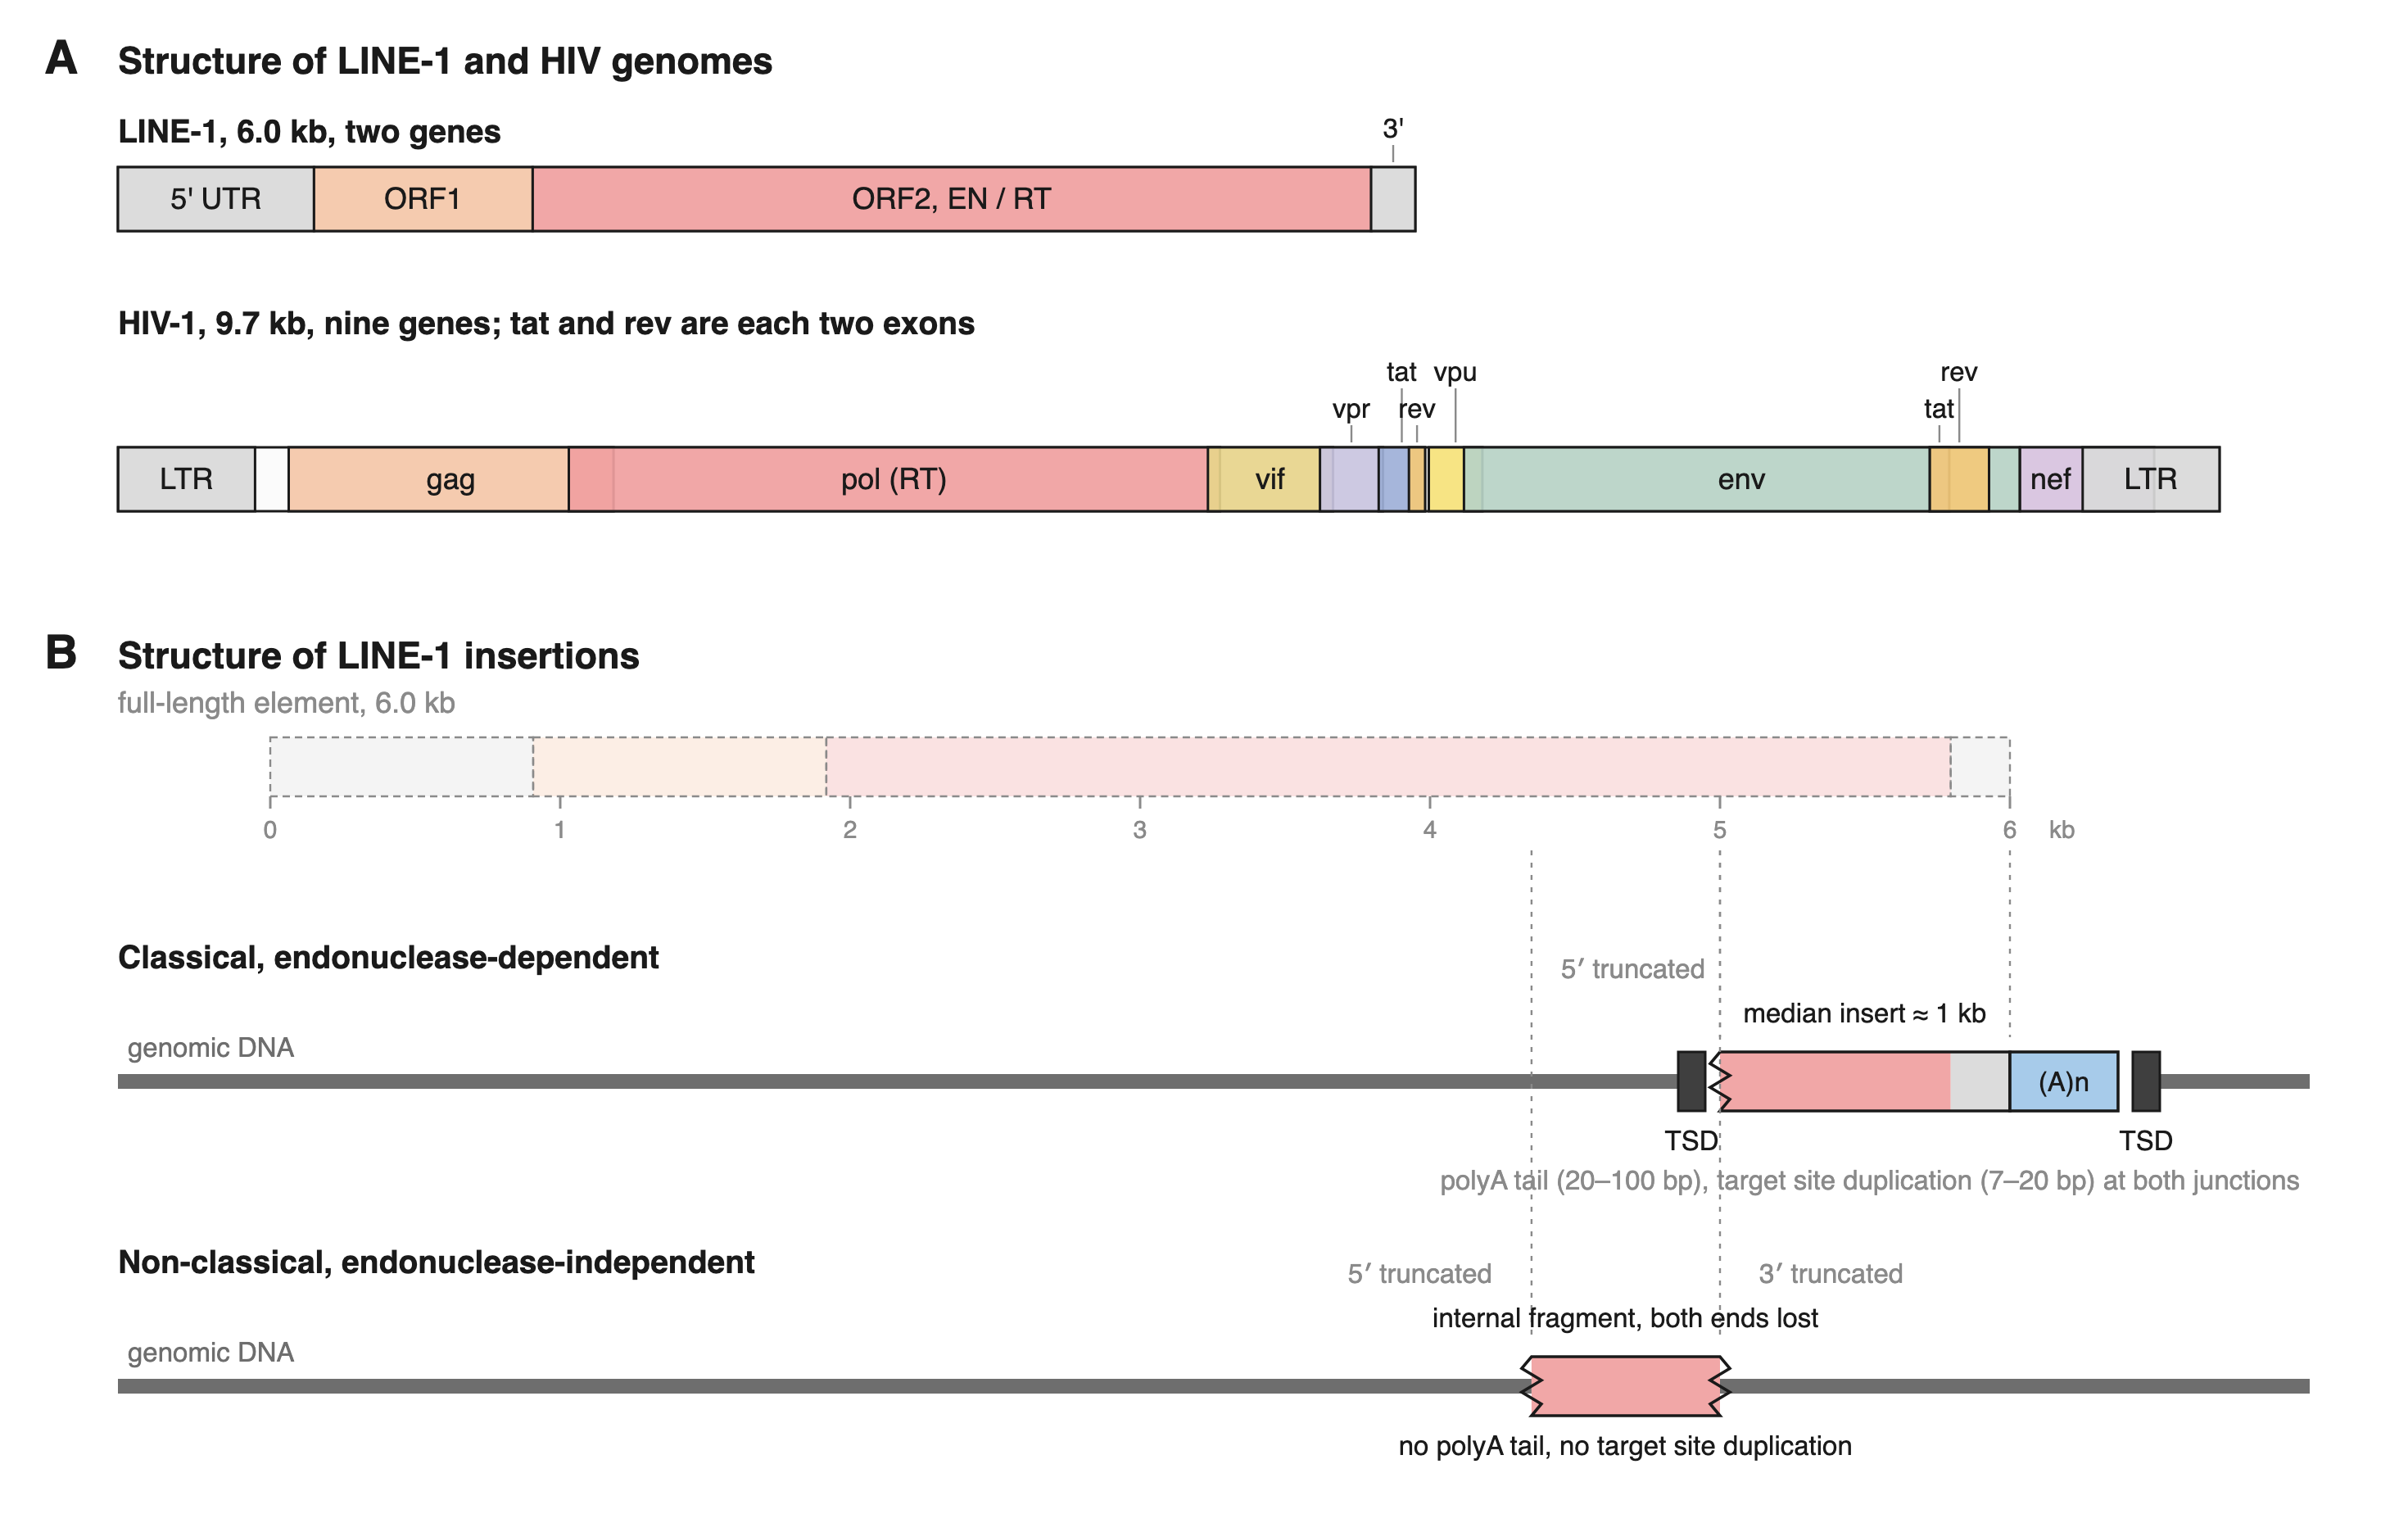
\includegraphics[width=0.77\textwidth]{../genomes.png}\par}
\caption{\textbf{LINE-1, HIV-1, and the two classes of insertion.}
\textbf{a}, LINE-1 is 6.0\,kb and encodes ORF1p and ORF2p (endonuclease and reverse transcriptase). HIV-1 is 9.7\,kb; reverse transcriptase is in \textit{pol}.
\textbf{b}, Classical, endonuclease-dependent insertions are usually 5$'$ truncated and retain a polyA tail and target-site duplications. Non-classical, endonuclease-independent insertions are truncated at both ends and have neither.}
\label{fig:genomes}
\end{figure*}

LINE-1 can also disrupt the functions of genes and contribute to genome instability. Successful insertions in the same orientation of genes inside their introns can introduce cryptic splice sites, polyadenylation signals, or otherwise impact gene expression\cite{perepelitsa}. Insertions fixed in the population are depleted in that orientation. The depletion is a previous result: young Ta-1 elements inside genes are antisense about twice as often as they are sense\cite{boissinot}, the bias is already present when the element inserts, and selection makes it stronger\cite{sultana}. Counted again on hg38, the short L1HS copies selection has barely touched are balanced, 425 sense and 432 antisense below 1\,kb, so a new insertion is taken to land sense half the time. The sense copies missing at longer lengths are the ones removed. Weighted by the length of young antisense insertions, and by the chance an insertion lands in an intron or in coding sequence, retrotransposition is 11\% of new coding loss-of-function alleles while only the youngest families are used, and 14\% when the deficit is taken from the family selection has purged most completely. Against the 0.07 protein-truncating variants counted per child in exome studies, the same two rates are 5\% and 6\%. The inputs are in the Methods. Furthermore, insertions inside exons of genes disrupt the gene completely\cite{cajuso}. Failed insertions leave a scar of small insertion/deletion events\cite{zhang}. They can cause more complex rearrangements such as reciprocal translocations between two chromosomes, or inversions of sequence\cite{zumalave,mendez}. This genome instability can generate further structural rearrangements such as deletions and duplications, complex rearrangements or DNA fragmentation, which is important in cancer\cite{mendez}. Retrotransposons are not the only factor influencing genome integrity. However, the damage they cause can contribute to both apoptosis and cell death as well as to cancer evolution, as we shall see in later sections.

\section{How does LINE-1 contribute to disease?}
LINE-1 is heavily suppressed in healthy adult cells through regulation of gene expression, sensing and degradation of foreign DNA, autophagy and breakdown of ribonucleoproteins, repair of DNA damage, triggering of cell death or apoptosis\cite{goodier2016}. Many different diseases involve dysregulation of genes involved in these processes. LINE-1 is likely not the initiating factor of any disease but is instead a downstream consequence that can contribute to disease progression. The ORF2p protein of LINE-1 is so toxic to cells that scientists were only recently able to produce enough of it to determine its 3D structure\cite{leslie}. Genome sequencing has revealed elevated levels of LINE-1 insertions into DNA in both cancer and neurological disorders\cite{rodriguez,jacob}.

\section{LINE-1's role in disease}
Independent studies have implicated LINE-1 in many diseases (Table~\ref{tab:diseases}). These include cancers, autoimmune disorders, developmental disorders, infectious disease and degeneration. Like many viruses, LINE-1 is both inflammatory and a mutagen. However, everyone contains $>$100 potentially active copies.

\begin{table*}[!t]
\caption{\textbf{Diseases in which LINE-1 has been implicated.}
Gene is the host gene linked to LINE-1 activity. The mechanism is the route proposed in the cited work.}
\label{tab:diseases}
\vspace{0.3em}
\footnotesize
\setlength{\tabcolsep}{4pt}
\renewcommand{\arraystretch}{1.12}
\begin{tabularx}{\textwidth}{@{}>{\RaggedRight\arraybackslash}p{2.7cm} >{\RaggedRight\arraybackslash}p{3.15cm} >{\RaggedRight\arraybackslash}p{2.05cm} Y l@{}}
\toprule
\textbf{Disease} & \textbf{Category} & \textbf{Gene} & \textbf{LINE-1 mechanism} & \textbf{References} \\
\midrule
Senescence & Aging & RB1 & chromatin relaxation; accumulation of L1 cDNA & \cite{cecco,simon} \\
Progeroid syndromes & Aging & LMNA, SIRT6 & accumulation of L1 RNA; chromatin relaxation & \cite{simon,dellavalle} \\
Ataxia-telangiectasia & Neurodevelopmental & ATM & increased L1 retrotransposition & \cite{jacob,takahashi,coufal} \\
Rett syndrome & Neurodevelopmental & MECP2 & hypomethylation & \cite{jacob,martins} \\
Down syndrome & Neurodevelopmental &  & misregulated L1 expression & \cite{martinez} \\
Tuberous sclerosis & Neurodevelopmental & TSC1, TSC2 & mTOR growth signaling activates L1 & \cite{jacob,martin} \\
Cytomegalovirus & Infectious & TSC2 & mTOR growth signaling activates L1 & \cite{hwang} \\
Aicardi-Goutieres & Inflammatory & TREX1, SAMHD1 & accumulation of L1 cDNA & \cite{thomas,crow} \\
Fanconi anemia & Inflammatory & SLX4, FANCD2 & accumulation of L1 cDNA & \cite{bregnard} \\
Sterile inflammation & Inflammatory & CGAS, STING1 & accumulation of L1 cDNA & \cite{cecco} \\
Lupus & Autoimmune & TREX1 & demethylation; accumulation of L1 RNA & \cite{mavragani} \\
GI, lung, head \& neck, ovarian, liver & Oncological & TP53 & demethylation & \cite{rodriguez,gasior,zhang,mendez,rajurkar,mendez2} \\
Chemo / radiotherapy & Oncological & TP53 & stress-induced activation & \cite{rajurkar} \\
ALS / FTD & Neurodegenerative & TARDBP & chromatin relaxation & \cite{liu} \\
Alzheimer / tauopathy & Neurodegenerative & MAPT & chromatin relaxation & \cite{herdy} \\
Parkinson's & Neurodegenerative &  & L1 activation in substantia nigra, putamen and microglia & \cite{garza,gordillo} \\
Geographic atrophy & Degenerative & DICER1 & L1 reverse transcription of Alu RNA & \cite{fukuda} \\
\bottomrule
\end{tabularx}
\end{table*}

LINE-1 inhibitors have slowed progression of otherwise unrelated diseases in preclinical studies, including cancer\cite{rajurkar,novototskaya}, progeroid syndromes\cite{simon,dellavalle}, Rett syndrome\cite{martins}, Ataxia-Telangiectasia\cite{takahashi}, Aicardi-Goutieres syndrome (AGS)\cite{thomas}, Down's syndrome\cite{martinez}, Alzheimer's\cite{herdy}, and non-infectious (sterile) inflammation\cite{cecco}.

What is not yet resolved is the relative contribution of LINE-1 to each disease. Many studies use indirect methods such as signatures of inflammation or LINE-1 mRNA expression, which are challenging to attribute to elevated retrotransposition accurately\cite{faulkner}. Whole-genome sequencing has identified elevation of LINE-1 insertions in post-mortem or biopsied brain tissue of individuals with Ataxia-Telangiectasia, Tuberous Sclerosis, and Rett Syndrome\cite{jacob}. It is also controversial how much LINE-1 activation occurs in the brain\cite{jacob,upton,erwin,evrony}. To accurately measure this requires single-nucleus whole-genome sequencing of post-mortem brain tissue. Novel computational biology algorithms are required, such as retrotransposon-miner (\href{https://github.com/L1-Therapeutics/retrotransposon-miner}{\faGithub}~\url{https://github.com/L1-Therapeutics/retrotransposon-miner}).

Another unresolved issue is determining when it is possible to intervene during the course of disease progression. It is possible to measure LINE-1 in real-time in cancer because dying cancer cells release LINE-1 ORF1p protein. However, for neurological disorders or diseases of aging this requires retrospective studies of diseased tissue.

Furthermore, LINE-1 is not the only contributor to inflammation. LINE-1 induced cell-death / degeneration cannot be reversed. Also LINE-1 mutations insert unpredictably and are not the only mutagenic factor in cancer or cell death. LINE-1 inhibitors are not a cure for any disease, however they are likely a necessary, but not sufficient piece of the puzzle. They would be used as an anti-inflammatory, or prophylactically to preserve genome stability over a period of years. But the long timelines of disease progression make it both costly and challenging to measure benefits in a traditional clinical trial setting.

In spite of promising preclinical studies, there has not yet been a successful clinical trial for reverse transcriptase inhibitors. Censavudine has been tested in a phase 2 clinical trial against LINE-1 for amyotrophic lateral sclerosis (ALS) (NCT04993755), Lamivudine for colorectal cancer (NCT03144804)\cite{rajurkar}, and a combination of inhibitors for Aicardi-Goutieres syndrome\cite{crow}. We shall learn in the next section theoretical reasons why these trials may not have been as successful as investigators expected.

\section{Therapeutic Strategies for LINE-1}
Three strategies have been proposed for LINE-1, antisense oligonucleotides (ASOs), ORF2p endonuclease inhibitors and ORF2p reverse transcriptase inhibitors\cite{dellavalle,dordine,jones,dai}. Other approaches include cancer vaccines against ORF1p\cite{mckerrow}. However, they will not be discussed here.

\subsection{Reverse transcriptase inhibitors (RTIs)}
Reverse transcriptase inhibitors are analogues of nucleosides, the building blocks of DNA. There are nucleoside inhibitors for each nucleoside; adenosine, cytidine, thymidine and guanosine. The potency of RTIs for HIV correlates strongly with their potency for LINE-1 (Figure~\ref{fig:nrti}A). On the 18 nucleosides with an exact value for both, the log$_{10}$ fit has slope 0.84 and Pearson $r = 0.89$ (Spearman $\rho = 0.90$). Restating each IC$_{50}$ per 1,000 template bases, using the sequences in the Methods, leaves the fit at slope 0.82 and $r = 0.88$ ($\rho = 0.91$). Alimatravir has no published LINE-1 IC$_{50}$. The 100-nt line in Figure~\ref{fig:nrti}C is the HIV intracellular IC$_{50}$ rescaled by how many adenine-analogue sites that LINE-1 sequence contains. Retroviruses diverged evolutionarily from retrotransposons over a billion years ago\cite{aiewsakun}. However, both take deoxyribose nucleoside triphosphates (dNTPs) as substrates, which are unchanged since the dawn of life. Consequently, the shape of the active site of the enzyme has been preserved across evolutionary time\cite{baldwin}. This creates a vulnerability that nucleoside chemists have exploited to develop antivirals. The fact that antivirals work so consistently on HIV and LINE-1 reverse transcriptases, but not consistently on host enzymes that take dNTPs as substrates (such as mitochondrial polymerase gamma, telomerase, and DNA polymerase), is evidence of the shared origins of retroviruses and retrotransposons. However, LINE-1 requires higher dosing to be sufficiently inhibited, and approved HIV regimens are constructed to provide the minimum necessary dose to sufficiently inhibit HIV. Potency is not the only consideration, as molecules that do inhibit LINE-1 / HIV can also have off-target effects (Table~\ref{tab:nucleosides}), cross the blood-brain barrier with varying efficiency, be activated in only certain cell types, or have different half-lives.

\begin{figure*}[!t]
\noindent
\begin{minipage}[t]{\textwidth}
{\sffamily\bfseries A}\par\vspace{1pt}
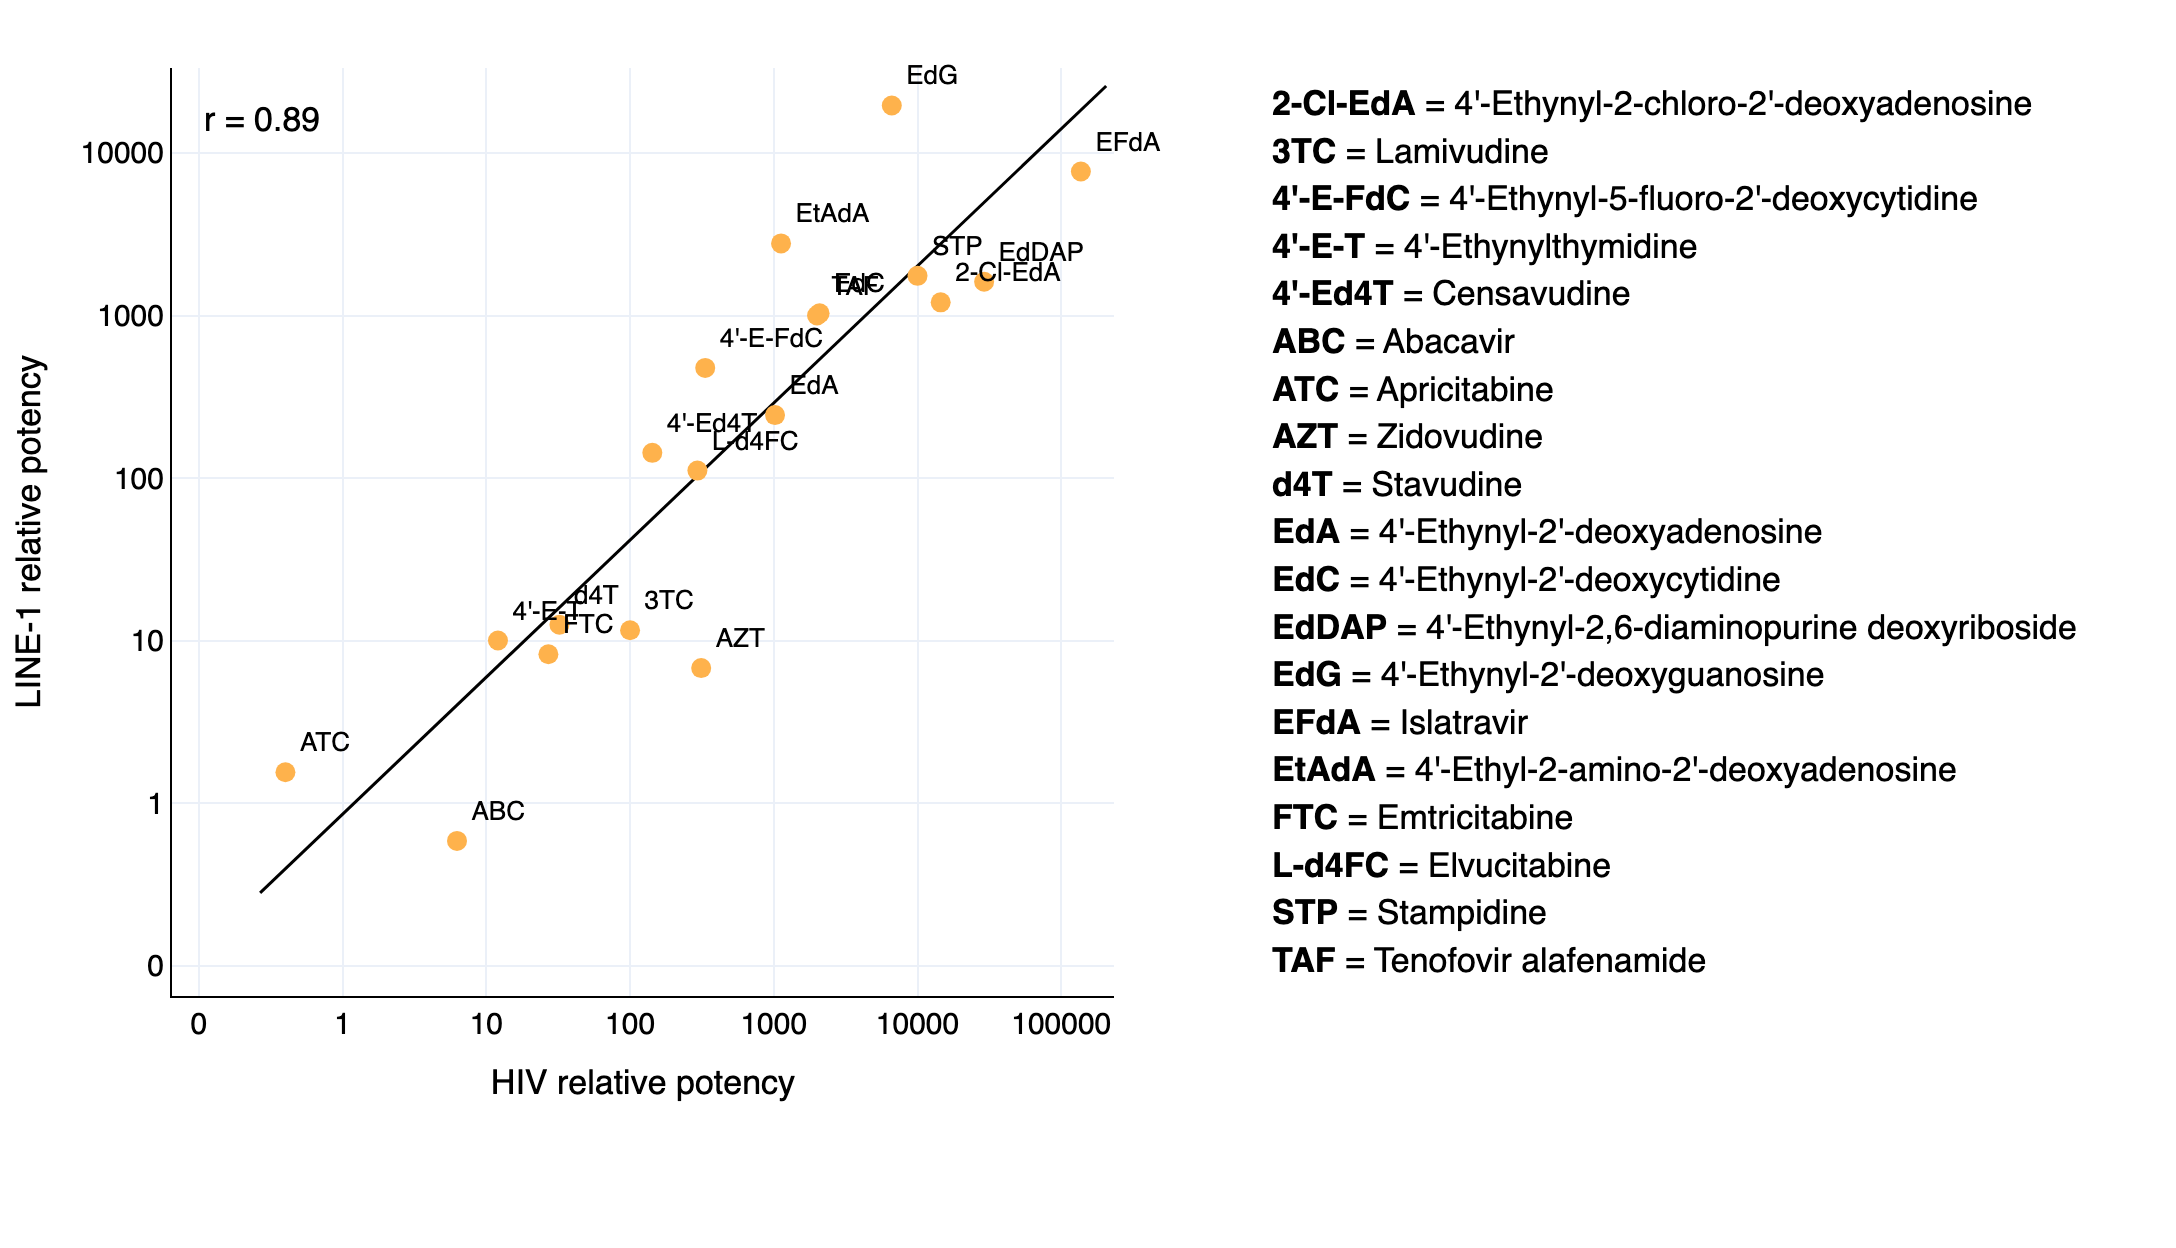
\includegraphics[width=\textwidth]{../line1_hiv_correlation.png}
\end{minipage}
\par\vspace{0.55em}
\noindent
\begin{minipage}[t]{0.34\textwidth}
{\sffamily\bfseries B}\par\vspace{1pt}
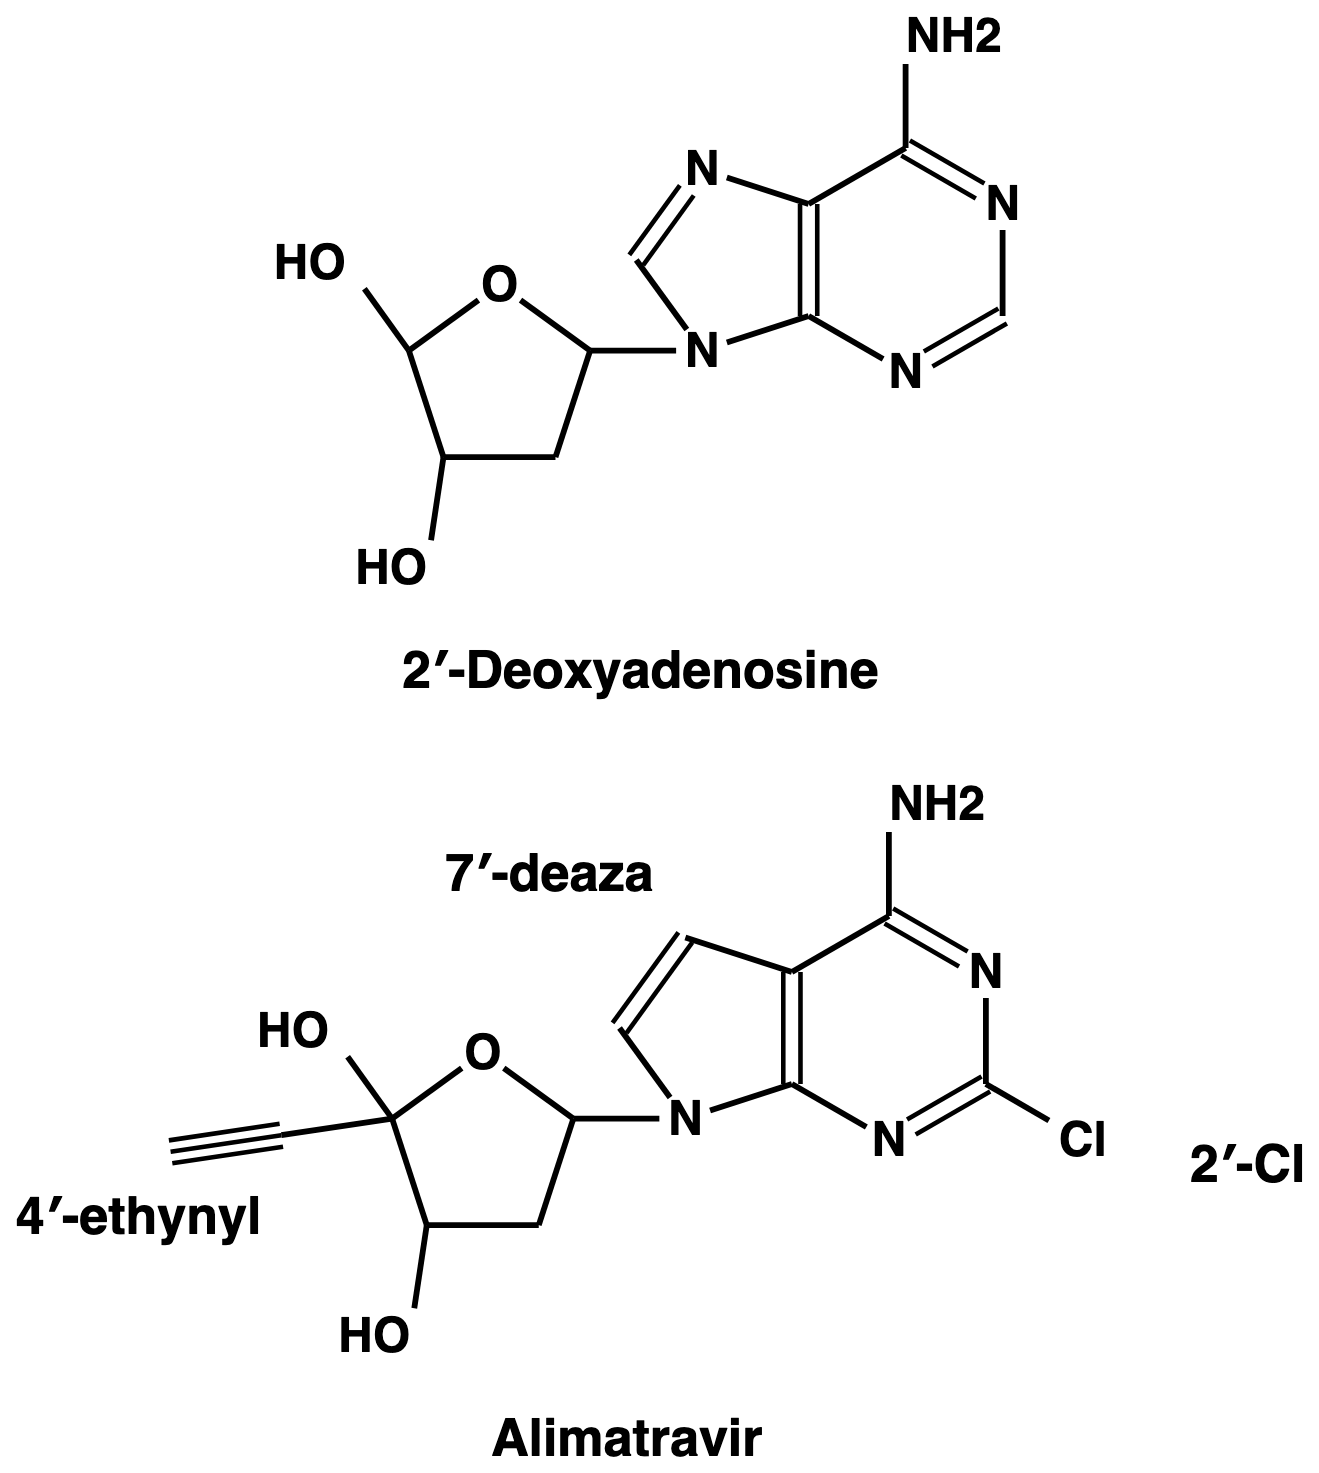
\includegraphics[width=\linewidth]{alimatravir_stacked.png}
\end{minipage}\hfill
\begin{minipage}[t]{0.63\textwidth}
{\sffamily\bfseries C}\par\vspace{1pt}
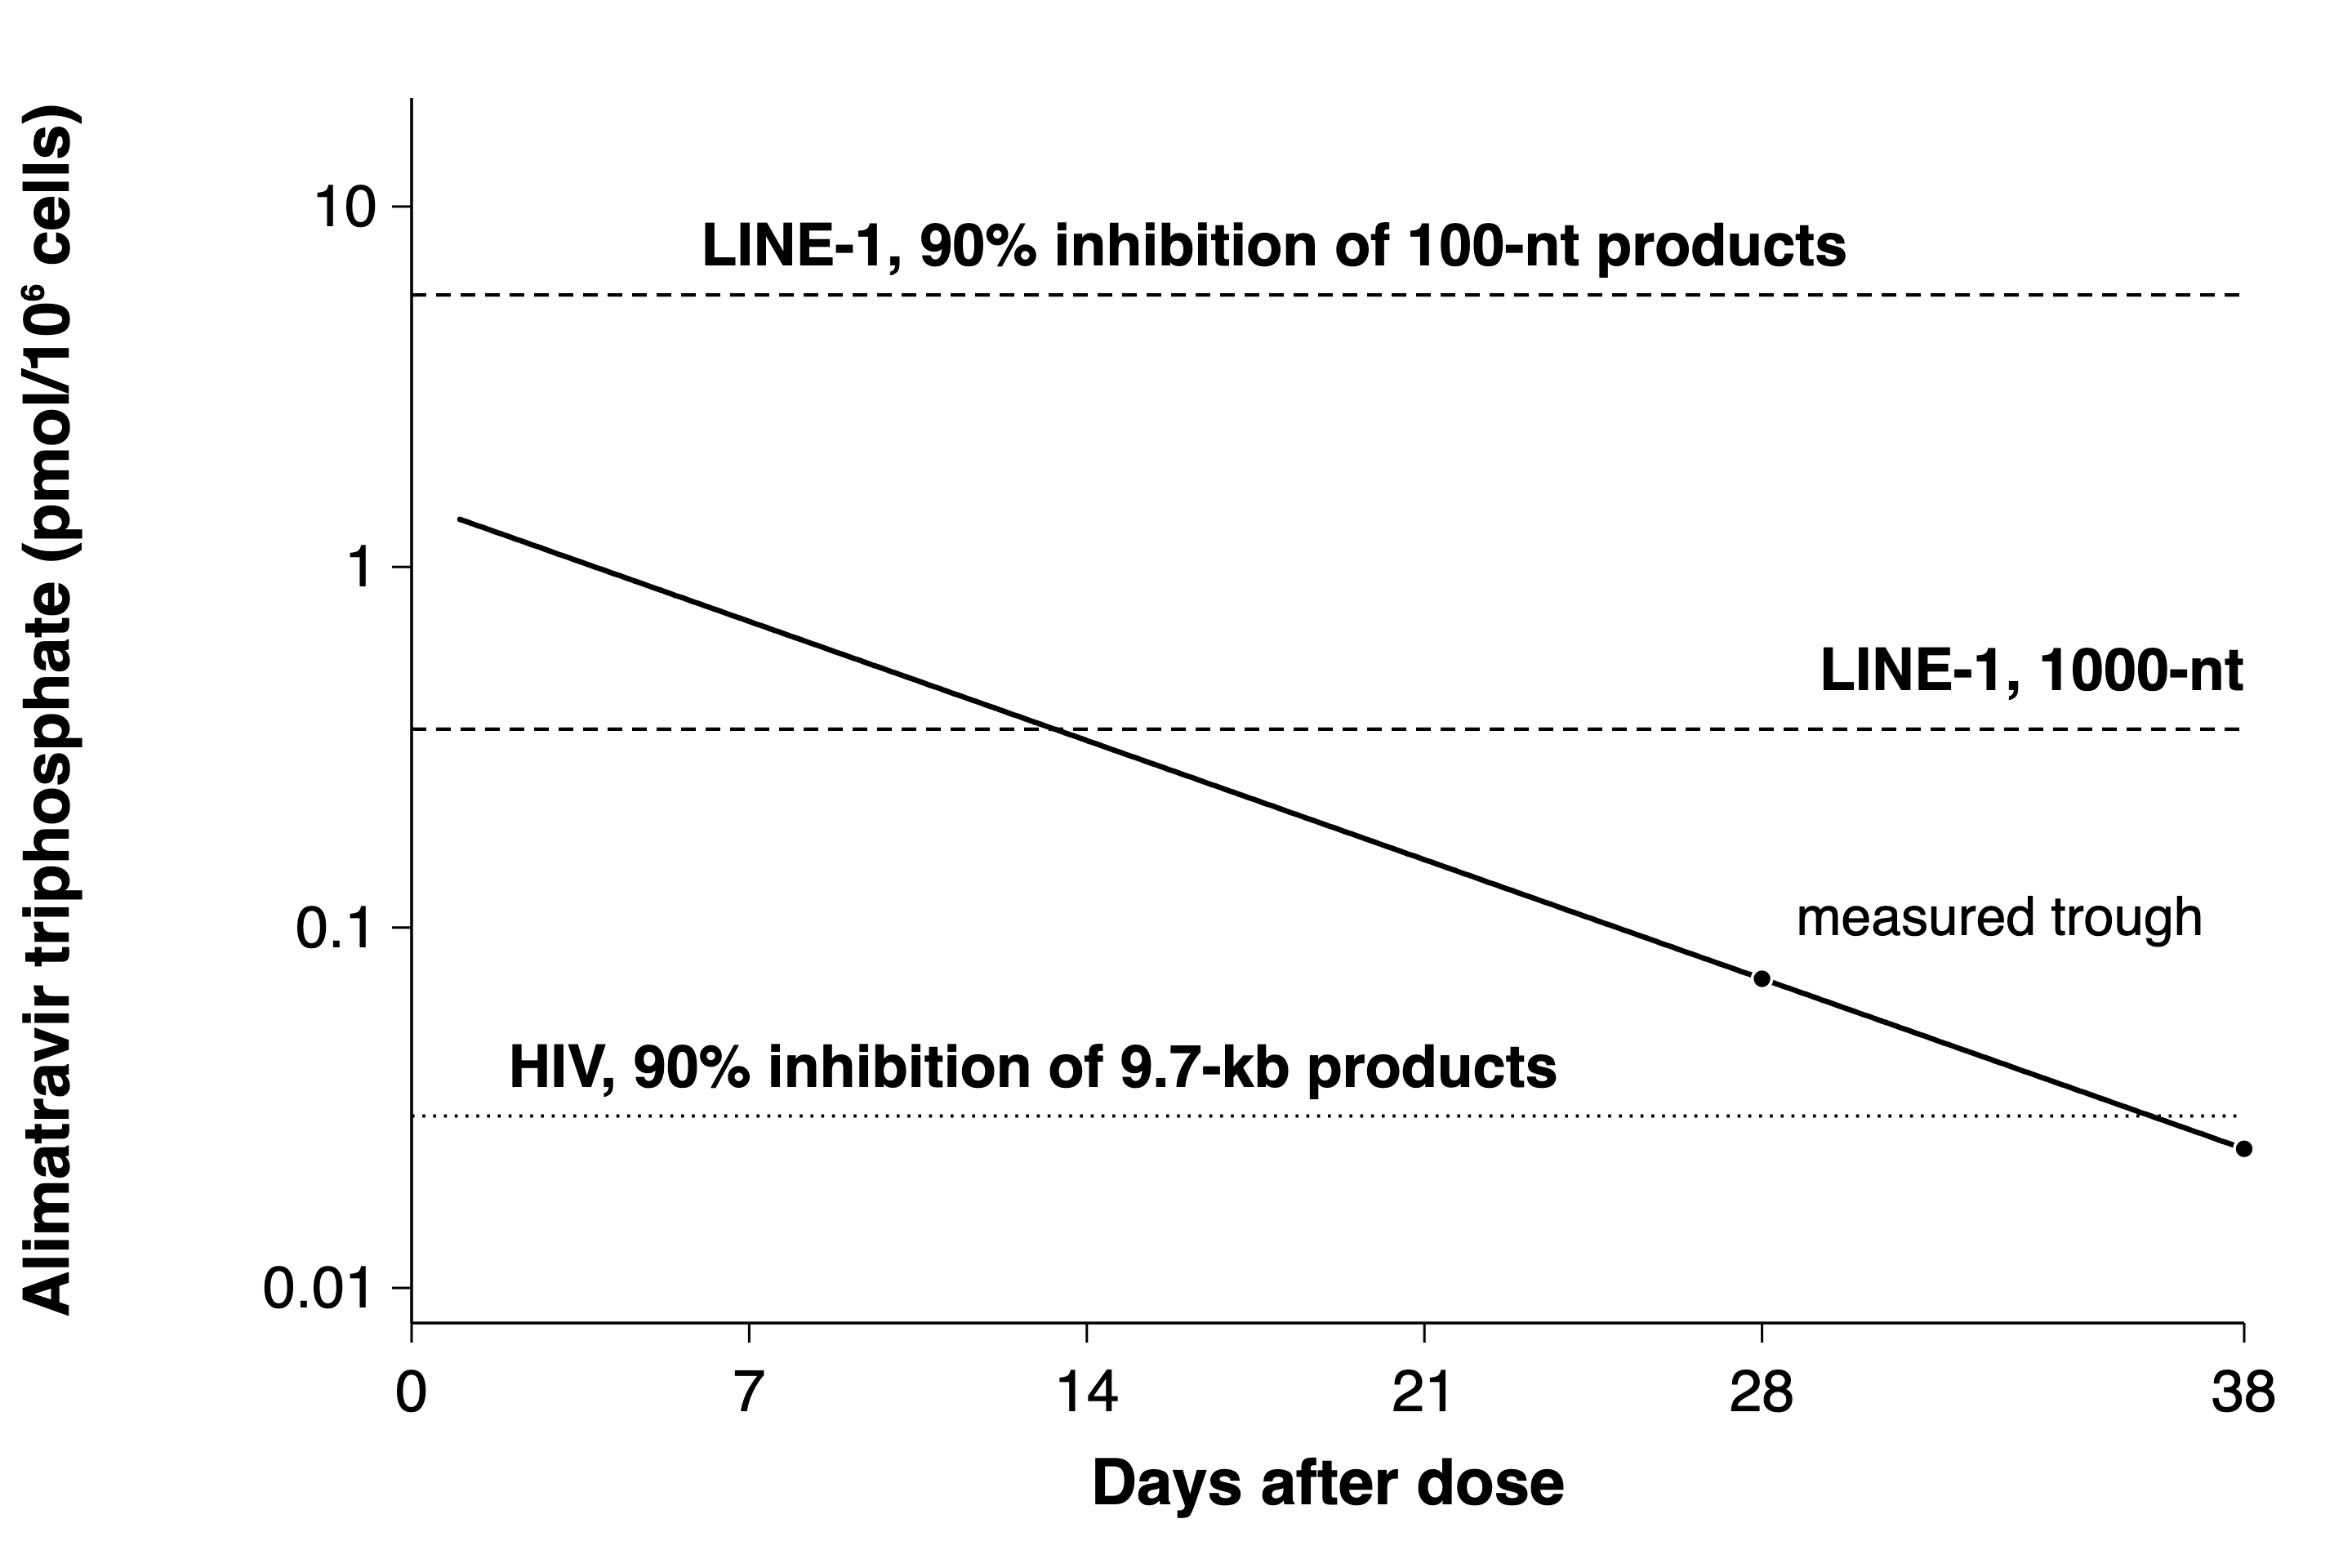
\includegraphics[width=\linewidth]{../alimatravir_11mg_decay.png}
\end{minipage}
\caption{\textbf{Nucleoside potency, structure, and exposure.}
\textbf{a}, Relative potency of nucleoside analogues. LINE-1 potency tracks HIV potency.
\textbf{b}, Deoxyadenosine and alimatravir. Alimatravir is 2-chloro-7-deaza-4$'$-ethynyl-2$'$-deoxyadenosine.
\textbf{c}, Intracellular alimatravir triphosphate after one 11\,mg oral dose, in pmol per 10$^{6}$ peripheral blood mononuclear cells, on a logarithmic scale. The upper LINE-1 line is 90\% inhibition of a 100-nt product, scaled from the HIV intracellular IC$_{50}$ by the number of adenine-analogue sites in the pYX017 cassette (Methods). The middle line is the same calculation for a 1,000-nt product. The lower line is 90\% inhibition of a 9.7\,kb HIV product.
Data are from US20240173346A1, US20230293526A1, US20240366649A1, US20260035403A1, US12187758B2, EP1177202B1\cite{raheem,kawamoto,kodama,takamatsu,lin,nitanda,hachiya,parkin,mayer}.}
\label{fig:nrti}
\end{figure*}

\begin{table*}[!t]
\caption{\textbf{Nucleoside analogues tested on LINE-1 and HIV.}
Concentrations are nM.}
\label{tab:nucleosides}
\vspace{0.25em}
\scriptsize
\setlength{\tabcolsep}{3.2pt}
\renewcommand{\arraystretch}{1.08}
\centering
\begin{tabular}{@{}>{\raggedright\arraybackslash}p{6.05cm} l c r r r r r r@{}}
\toprule
\textbf{Compound} & \textbf{Short} & \textbf{Base} & \textbf{LINE-1 IC$_{50}$} & \textbf{HIV EC$_{50}$} & \textbf{CC$_{50}$} & \textbf{Pol $\gamma$} & \textbf{Pol $\alpha$} & \textbf{Telomerase} \\
\midrule
Alimatravir & MK-8527 & A &  & 0.21 & $>$42,000 & $>$200,000 & 95,000 &  \\
Islatravir & EFdA & A & 1.3 & 0.073 & 7,500 & 10,000 & $>$100,000 &  \\
4$'$-Ethynyl-2$'$-deoxyguanosine & EdG & G & 0.51 & 1.51 & 1,400 &  &  &  \\
4$'$-Ethynyl-2,6-diaminopurine deoxyriboside & EdDAP & A & 6.2 & 0.344 & 900 &  &  &  \\
4$'$-Ethyl-2-amino-2$'$-deoxyadenosine & EtAdA & A & 3.6 & 8.9 & 35,900 &  &  &  \\
4$'$-Ethynyl-2$'$-deoxycytidine & EdC & C & 9.7 & 4.8 & 2,200 &  &  &  \\
Tenofovir alafenamide & TAF & A & 10 & 5 & 4,700 &  &  & 13,000 \\
ROME compound I-1 & I-1 & A & 8.3 &  & $>$100,000 &  &  &  \\
4$'$-vinyl-5-fluoro-2$'$-deoxycytidine & ROME-74 & C & 9 &  & $>$100,000 &  &  &  \\
4$'$-vinyl-2$'$-deoxyguanosine & ROME-69 & G & 13 &  & 5,500 &  &  &  \\
4$'$-Ethynyl-5-fluoro-2$'$-deoxycytidine & 4$'$-E-FdC & C & 21 & 30 & $>$100,000 &  &  &  \\
4$'$-chloromethyl-2$'$-deoxycytidine & ROME-2 & C & $<$50 &  & $>$100,000 & $\leq$50,000 &  & $\leq$1,000 \\
2$'$-fluoro-4$'$-chloromethyl-5-fluoro-2$'$-deoxycytidine & ROME-67 & C & $<$50 &  & $>$100,000 & 250,000 &  & $>$100,000 \\
Elvucitabine & L-d4FC & C & 90 & 34 &  &  &  &  \\
Censavudine & 4$'$-Ed4T & T & 70 & 70 & $>$100,000 & 100,000 & $>$100,000 &  \\
Lamivudine & 3TC & C & 640 & 100 & $>$100,000 &  &  & $>$150,000 \\
Zidovudine & AZT & T & 810 & 32 & 29,000 &  &  & 46,000 \\
Stavudine & d4T & T & 750 & 310 & 79,000 & 1,000 &  & 15,000 \\
Emtricitabine & FTC & C & 1,340 & 370 &  &  &  & $>$150,000 \\
4$'$-Ethynylthymidine & 4$'$-E-T & T & $>$1,000 & 830 & $>$400,000 &  &  &  \\
Abacavir & ABC & G & 17,100 & 1,600 &  &  &  & 9,000 \\
\bottomrule
\end{tabular}
\par\vspace{0.35em}
{\raggedright\footnotesize Data are from US20240173346A1, US20230293526A1, US20240366649A1, US20260035403A1, US12187758B2, EP1177202B1\cite{raheem,kawamoto,kodama,takamatsu,lin,nitanda,hachiya,parkin,ohrui,nakata,haraguchi,yangpol,baldwin,callebaut}.\par}
\end{table*}

\subsubsection{Adenosine}
Adenosine analogues have specific modifications that prevent their metabolism and increase their selectivity for HIV.

The adenosine analogue with the widest therapeutic window and longest half-life Alimatravir (2-Chloro-7-deaza-4$'$-ethynyl-2$'$-deoxyadenosine; Table~\ref{tab:nucleosides}; Figure~\ref{fig:nrti}B)\cite{raheem,michailidis}. It is in Phase 3 for monthly dosing as pre-exposure prophylaxis (PrEP). A dose of just 11mg is sufficient to maintain $>$90\% suppression of HIV for one month in peripheral blood cells (Figure~\ref{fig:nrti}C). For the first few days the dose is also theoretically high enough to suppress $>$90\% of 100 nucleotide LINE-1 products in the periphery of the body (Figure~\ref{fig:nrti}C).

There are three modifications to the bare nucleoside of Alimatravir that enable its high therapeutic index and long half-life. A 2$'$ chlorine on the adenine base prevents adenosine deaminase from metabolizing the nucleoside to inosine\cite{raheem}. The 4$'$ ethynyl group on the ribose sugar blocks SAMHD1 from breaking down the triphosphate, as well as incorporating more selectively into HIV/LINE-1\cite{michailidis}. Finally, the 7-deaza group prevents breakdown by purine nucleoside phosphorylase and also incorporation into host polymerases (Figure~\ref{fig:nrti}B)\cite{raheem}.

Adenine has two positions that can be altered while sparing Watson-Crick base pairing, whereas other bases only have one position that can be altered. Both of those positions are also used by catabolic enzymes to break down the nucleoside. Modifying them enables both a longer half life and selectivity for HIV / LINE-1.

There is no public data with a measurement for LINE-1 for Alimatravir. Nor is there data on its ability to cross the blood brain barrier. However, it is reasonable to assume the data will be similar to Islatravir (EFdA; Figure~\ref{fig:nrti}A), another adenosine analogue from the same series as Alimatravir, which does cross the blood brain barrier\cite{gillespie}.

\subsubsection{Thymidine}
When LINE-1 is reverse transcribed it starts copying the polyA tail of its messenger RNA, which is $\sim$40 nucleotides long and is complementary to thymidine (Figure~\ref{fig:genomes}). Thymidine analogues could in theory shut down LINE-1 reverse transcription before it is able to contribute to inflammation, which starts when it produces a product $>$45 nucleotides long\cite{andreeva}. Thymidine nucleosides primarily get activated by thymidine kinase. This enzyme is only present in dividing cells, as thymidine is required only for DNA (not for RNA). Whereas resting cells can synthesize dTTP as needed, rendering thymidine analogues potentially less effective in non-dividing cells such as neurons\cite{sherley}. Thymidine analogues therefore may be particularly beneficial in dividing cells such as in colorectal cancer, especially given the chemotherapy standard of care (SoC) leverages thymidine synthesis inhibitors (5-FU), which is rationally synergistic with thymidine analogues.

Mitochondria contain their own thymidine kinase, which can activate nucleosides and contribute to mitochondrial toxicity\cite{arner}. The thymidine analogue censavudine has a 4$'$ethynyl modification (like Alimatravir), which enables both a strong LINE-1 potency and orders of magnitude lower incorporation into mitochondrial polymerase gamma\cite{gupta}.

Unfortunately, the cell efficiently turns over thymidine-triphosphates. Thymidine is also cleared by thymidine phosphorylase cutting its glycosidic bond. Although Censavudine's 4$'$ethynyl resists this process, its half life is still much shorter than that of adenosine analogues such as Alimatravir. Censavudine has been used in a Phase 2 trial for amyotrophic lateral sclerosis / frontotemporal dementia (NCT04993755), and its lack of demonstrated efficacy may in part be due to lack of activation in neurons.

\subsubsection{Cytidine}
Two of the most commonly prescribed nucleosides for HIV are cytidine analogues, Lamivudine (3TC) and Emtricitabine (FTC). Although their potency is not as high as for other molecules, they have strong safety records due to having opposite chirality to natural nucleosides, alongside other modifications\cite{coates}. Lamivudine has been tested in a Phase 2 trial for stage IV colorectal cancer (NCT03144804), but did not have sufficient potency to affect the progression of the disease beyond what you would expect by chance\cite{rajurkar}. Lamivudine at standard doses is not potent enough to sufficiently suppress LINE-1. ROME therapeutics screened cytidine nucleosides for LINE-1, generating novel compounds that have greater potency than 3TC or FTC, and which may be in the same range as the adenosine analogues (ROME Therapeutics, US12187758B2; Table~\ref{tab:nucleosides}). However, their safety is not established. It is also unlikely that any are substantially more potent or safer than Alimatravir.

\subsubsection{Guanosine}
Guanosine analogues have historically had issues with toxicity. The most potent known nucleoside for LINE-1 is 4$'$-Ethynyl-2$'$-deoxyguanosine (0.51\,nM) (Table~\ref{tab:nucleosides}; Figure~\ref{fig:nrti}A). In six-week-old male mice, one dose of 4$'$-ethynyl-deoxyguanosine also killed every animal at 3 mg/kg within a few days\cite{ohrui}, but 1mg / kg did not. However, these are very high doses. Although highly potent (Figure~\ref{fig:nrti}A), none are approved for HIV. Deoxyguanosine analogues are phosphorylated mainly by mitochondrial deoxyguanosine kinase, which may contribute to toxicity due to proximity to mitochondrial polymerase gamma. Guanosine analogues are underexplored. However, LINE-1 is AT rich ($\sim$57\%) and adenosine and thymidine analogues are in theory better suited.

\subsubsection{Prodrug formulations}
Bare nucleosides of guanosine, cytidine and adenosine cannot easily be combined because they compete with each other for phosphorylation by cellular kinase enzymes\cite{arner}. In theory this is less problematic for the potent nucleosides, because the ratio of nucleoside to natural dNTPs is lower. Tenofovir alafenamide is a prodrug formulation that contains a phosphonate group that has been masked, enabling combinations of the nucleosides as the first phosphorylation step is not necessary. While potent for HIV and LINE-1\cite{callebaut} (Table~\ref{tab:nucleosides}), the downside of this approach is the prodrug formulations typically do not cross the blood-brain barrier\cite{best}. Also adenosines are readily phosphorylated, and both islatravir \& alimatravir are more potent and safer than TAF while being bare nucleosides (Table~\ref{tab:nucleosides}).

\subsection{ORF1p / ORF2p inhibitors}
Even if LINE-1 reverse transcription is completely shut down, this does not prevent LINE-1's ORF2p endonuclease domain from cutting DNA. This is so toxic to cells that scientists were not able to produce enough of the protein to determine its structure until 2023\cite{baldwin,leslie,thawani}. One attempt has been made to make a non-nucleoside inhibitor that inhibits the endonuclease domain of ORF2p\cite{dordine}. One challenge is that the endonuclease shares conserved catalytic sites with host DNA repair enzymes such as APE1. Just like with HIV, a combination of a reverse transcriptase inhibitor with a non-nucleoside small molecule inhibitor will be necessary to completely shut down LINE-1's activity.

\subsection{Antisense Oligonucleotides}
Antisense oligonucleotides (ASOs) could potentially prevent the translation of LINE-1 mRNA into ORF1p \& ORF2p. They have shown promise for LINE-1 in preclinical models of Hutchinson-Gilford progeria\cite{dellavalle} and Alzheimer's\cite{herdy}. However, LINE-1 is 17\% of the genome. It is not possible to design an ASO for LINE-1 that does not have hundreds of potential off-target effects in introns of pre-mRNA. There are two types of ASO, a gapmer, which is RNA with a DNA sequence in the middle that recruits RNase H to cut the bound RNA catalytically, and steric blockers, which occupy the target site, preventing translation. For gapmers, LINE-1 ASOs would also degrade potentially important coding genes. For steric blockers their effects would be diluted by off-target binding, requiring high doses. Short interfering RNAs (siRNAs) also present similar challenges of off-target effects.

\section{Future Perspectives}
The challenge with all diseases where LINE-1 is implicated is that treatment with inhibitors is not a cure for that disease, instead LINE-1 contributes to progression. For example, in cancer LINE-1 causes mutations that cause tumor evolution. But it is not the only source of mutations. The same is true for degeneration and inflammation. Furthermore, most studies in these diseases are somewhat preliminary, and we do not have a clear picture of the relative importance of LINE-1 to each disease it has been associated with, outside of cancer. New technologies such as single-nucleus whole-genome sequencing open the door to stack-ranking diseases by the prevalence of insertions in diseased tissue across a range of ages and disease stages. This requires novel computational biology algorithms, such as retrotransposon-miner (\href{https://github.com/L1-Therapeutics/retrotransposon-miner}{\faGithub}).

The market for many of these diseases individually is smaller than it is for HIV. Furthermore since LINE-1 touches such broad areas of aging and disease, learnings from one disease do not automatically translate to another. This makes it challenging to develop a therapeutic strategy to expand access to these medicines under the existing patent and regulatory frameworks.

The potency and safety of next generation reverse transcriptase inhibitors such as Alimatravir potentially enable their application to LINE-1. A higher dose or shorter dosing interval is still required for LINE-1 (Figure~\ref{fig:nrti}C). However, Alimatravir's monthly dose costs $\sim$\$1.80 to manufacture. This creates a challenge for the economics of expanding access for nucleosides to LINE-1. Because the cost of performing the necessary preclinical work and trials to determine when treatment would be effective far exceeds what can be recouped due to pricing pressure from off-label prescribing. Furthermore, method-of-use patents protecting the use of nucleosides for new diseases are too obvious to be considered an invention.

However, reverse transcriptase inhibitors alone are not sufficient for LINE-1, even at higher doses. One concern that has been raised about them is that stopping reverse transcriptase early can free up ORF2p endonuclease to repeatedly cut DNA\cite{rajurkar}. However, this is unlikely given that $>$10 DNA cuts are made for each successful insertion\cite{gasior}. Furthermore, ORF2p is unstable without RNA bound\cite{baldwin}, and reverse transcriptase inhibitors reduce DNA damage rather than increasing it\cite{dordine}. Also, the success of reverse transcriptase inhibitors outside of cancer in preclinical studies argues against this hypothesis.

Regardless, a combination of inhibitors will be required for LINE-1 because reverse transcriptase inhibitors only partially prevent DNA damage\cite{dordine}. Therefore, a reverse transcriptase inhibitor and at least one additional inhibitor that blocks endonuclease activity or degrades the protein. As of the date of this publication, there are no announced therapeutic programs targeting LINE-1 through ORF2p inhibition outside of reverse transcriptase inhibitors.

\section{Methods}
\subsection{Intronic orientation and the loss-of-function rate}
RepeatMasker annotations were the UCSC hg38 rmsk table. Introns are autosomal protein-coding gene spans in GENCODE v50 minus every annotated exon of those genes, so a base counted as intronic is intronic on that strand in every overlapping protein-coding transcript. An element is sense when its strand matches the gene at the element's midpoint, and antisense when it does not. Copies whose midpoint falls in an intron on both strands are left out. Chromosomes X and Y are left out, because the gnomAD table used as the denominator has no rows there.

The probability a new insertion is sense is one half. That is the short-L1HS count above, not an assumption carried over from the earlier Ta-1 surveys. In a length bin the sense deficit is one minus the ratio of sense copies to antisense copies, which is the fraction of sense insertions in that bin that selection removed. The length spectrum of a new insertion is the length distribution of antisense copies of the youngest family in the class, the copies selection has barely touched. Two brackets are reported. The young bracket weights the deficit of L1HS, AluY, or SVA by that spectrum. The other bracket uses the same spectrum and the most depleted family of the class, L1M for LINE-1 and AluS for Alu. SVA has one family in this annotation, so the two brackets are the same for SVA.

The probability that one insertion is a loss-of-function allele is the probability it lands in a protein-coding intron, times one half, times the deficit, plus the probability it lands in coding sequence. The intron probability is read from the antisense copies of the youngest family, which carries the element's own insertion preference, and is then multiplied by the autosomal share of the assembly. Published de novo rates supply the insertions per birth: about 1 in 100 for LINE-1, 1 in 20 for Alu, and 1 in 900 for SVA\cite{hancks,ewing,xing}. The denominator is the sum of gnomAD v4.1 per-gene loss-of-function mutation rates over MANE Select genes with at least ten annotated loss-of-function sites, doubled for a diploid birth\cite{chen}, with frameshift indels added at one third of that point-mutation rate\cite{kaplanis}. The second denominator is the 0.07 de novo protein-truncating variants counted per child in the same exome catalogs\cite{kaplanis}.

\subsection{LINE-1 potency from the reporter sequence}
The LINE-1 cell IC$_{50}$s were measured in HeLa cells with reporter plasmid pYX017, in which firefly luciferase reports a completed retrotransposition\cite{xie}. The sequence that plasmid has to reverse transcribe before the assay scores is not the full 6\,kb element. It is 150\,bp from the 3$'$ end of L1.3, taken from GenBank L19088, a 40-base polyA, and the 1,653\,bp firefly luciferase coding sequence, 1,843\,bp in all. On that sequence the bases are A 591, T 497, G 394, and C 361. The HIV genome the comparator assays have to finish is HXB2, GenBank K03455, 9,719\,bp (A 3,411, T 2,163, G 2,373, C 1,772). An analogue is inserted opposite its complement, so an adenine analogue is scored on T.

Relative potency in Figure~\ref{fig:nrti}A is 100\,$\mu$M divided by the IC$_{50}$. Where more than one LINE-1 assay reported a nucleoside, the point is their geometric mean. The per-kilobase fit divides each IC$_{50}$ by the template length in kilobases before that ratio is taken. Eighteen nucleosides with an exact IC$_{50}$ on both targets enter the log$_{10}$ fit. 4$'$-Ethynylthymidine is censored, LINE-1 above 1\,$\mu$M, and stays out of the fit.

Alimatravir has no published LINE-1 IC$_{50}$. Its intracellular HIV IC$_{50}$ is 9.2\,fmol per 10$^{6}$ peripheral blood mononuclear cells\cite{raheem}, and that concentration is taken as the amount that stops half the copies of the 1,843\,bp cassette. One incorporation is treated as aborting the copy, so the concentration at which a fraction $s$ of copies finish scales as $-\ln s$ divided by the number of incorporation sites. For a 100-nt LINE-1 product the copied stretch is the 40-base polyA plus 60 bases of element. The polyA is copied with thymidine and contributes no site for an adenine analogue. The 60 bases carry T at the density of the 1,803 non-polyA bases, $497 \times 60/1{,}803$. Ninety percent inhibition is the concentration at which one tenth of those short products finish. The curve in Figure~\ref{fig:nrti}C is the intracellular triphosphate after one 11\,mg dose: the phase 2 geometric-mean peak after 12\,mg, and the mean of the week 8, 12, 16, and 24 troughs, each scaled by 11/12\cite{mayer}. The half-life is the single exponential joining that peak, placed at day 1, to that trough. The HIV line on the same panel is the published threshold of 0.03\,pmol per 10$^{6}$ cells.

\section{Competing interests}
W.B. is founder and chief executive of L1 Therapeutics, which develops therapeutics that inhibit LINE-1. The retrotransposon-miner software cited in this article is developed by L1 Therapeutics.

\FloatBarrier
\begin{thebibliography}{99}
\footnotesize
\setlength{\itemsep}{0.12em}
\setlength{\parsep}{0pt}

\bibitem{dong} Dong, X., Milholland, B. \& Vijg, J. Evidence for a limit to human lifespan. \textit{Nature} \textbf{538}, 257--259 (2016).

\bibitem{cecco} Cecco, M. D. et al. LINE-1 derepression in senescent cells triggers interferon and inflammaging. \textit{Nature} \textbf{566}, 73--78 (2019).

\bibitem{rodriguez} Rodriguez-Martin, B. et al. Pan-cancer analysis of whole genomes identifies driver rearrangements promoted by LINE-1 retrotransposition. \textit{Nat. Genet.} \textbf{52}, 306--319 (2020).

\bibitem{gasior} Gasior, S. L., Wakeman, T. P., Xu, B. \& Deininger, P. L. The human LINE-1 retrotransposon creates DNA double-strand breaks. \textit{J. Mol. Biol.} \textbf{357}, 1383--1393 (2006).

\bibitem{ivancevic} Ivancevic, A. M., Kortschak, R. D., Bertozzi, T. \& Adelson, D. L. LINEs between Species: Evolutionary Dynamics of LINE-1 Retrotransposons across the Eukaryotic Tree of Life. \textit{Genome Biol. Evol.} \textbf{8}, 3301--3322 (2016).

\bibitem{goodier2001} Goodier, J. L., Ostertag, E. M., Du, K. \& Kazazian, H. H. A novel active L1 retrotransposon subfamily in the mouse. \textit{Genome Res.} \textbf{11}, 1677--1685 (2001).

\bibitem{beck} Beck, C. R. et al. LINE-1 Retrotransposition Activity in Human Genomes. \textit{Cell} \textbf{141}, 1159--1170 (2010).

\bibitem{baldwin} Baldwin, E. T. et al. Structures, functions and adaptations of the human LINE-1 ORF2 protein. \textit{Nature} \textbf{626}, 194--206 (2024).

\bibitem{morrish} Morrish, T. A. et al. DNA repair mediated by endonuclease-independent LINE-1 retrotransposition. \textit{Nat. Genet.} \textbf{31}, 159--165 (2002).

\bibitem{jacob} Jacob-Hirsch, J. et al. Whole-genome sequencing reveals principles of brain retrotransposition in neurodevelopmental disorders. \textit{Cell Res.} \textbf{28}, 187--203 (2018).

\bibitem{perepelitsa} Perepelitsa-Belancio, V. \& Deininger, P. RNA truncation by premature polyadenylation attenuates human mobile element activity. \textit{Nat. Genet.} \textbf{35}, 363--366 (2003).

\bibitem{cajuso} Cajuso, T. et al. Retrotransposon insertions can initiate colorectal cancer and are associated with poor survival. \textit{Nat. Commun.} \textbf{10}, 4022 (2019).

\bibitem{zhang} Zhang, T. et al. Uncovering the role of LINE-1 in the evolution of lung adenocarcinoma. \textit{Nature} 1--12 (2025) doi:10.1038/s41586-025-09825-y.

\bibitem{zumalave} Zumalave, S. et al. Concurrent L1 retrotransposition events promote reciprocal translocations in human tumorigenesis. \textit{Science} \textbf{392}, eaee4513 (2026).

\bibitem{mendez} Mendez-Dorantes, C. et al. Chromosomal rearrangements and instability caused by the LINE-1 retrotransposon. \textit{bioRxiv} 2024.12.14.628481 (2024) doi:10.1101/2024.12.14.628481.

\bibitem{goodier2016} Goodier, J. L. Restricting retrotransposons: a review. \textit{Mob. DNA} \textbf{7}, 16 (2016).

\bibitem{leslie} Leslie, M. Risky moves. \textit{Science} \textbf{388}, 244--247 (2025).

\bibitem{rajurkar} Rajurkar, M. et al. Reverse Transcriptase Inhibition Disrupts Repeat Element Life Cycle in Colorectal Cancer. \textit{Cancer Discov.} \textbf{12}, 1462--1481 (2022).

\bibitem{novototskaya} Novototskaya-Vlasova, K. A. et al. Inflammatory response to retrotransposons drives tumor drug resistance that can be prevented by reverse transcriptase inhibitors. \textit{Proc. Natl. Acad. Sci. U. S. A.} \textbf{119}, e2213146119 (2022).

\bibitem{simon} Simon, M. et al. LINE1 Derepression in Aged Wild-Type and SIRT6-Deficient Mice Drives Inflammation. \textit{Cell Metab.} \textbf{29}, 871--885.e5 (2019).

\bibitem{dellavalle} Della Valle, F. et al. LINE-1 RNA causes heterochromatin erosion and is a target for amelioration of senescent phenotypes in progeroid syndromes. \textit{Sci. Transl. Med.} \textbf{14}, eabl6057 (2022).

\bibitem{martins} Martins, A. M. A. et al. Dormant viral pathways underlie space-induced neural senescence. 2025.11.02.686043 Preprint at \url{https://doi.org/10.1101/2025.11.02.686043} (2026).

\bibitem{takahashi} Takahashi, T. et al. LINE-1 activation in the cerebellum drives ataxia. \textit{Neuron} \textbf{110}, 3278--3287.e8 (2022).

\bibitem{thomas} Thomas, C. A. et al. Modeling of TREX1-Dependent Autoimmune Disease using Human Stem Cells Highlights L1 Accumulation as a Source of Neuroinflammation. \textit{Cell Stem Cell} \textbf{21}, 319--331.e8 (2017).

\bibitem{martinez} Martinez de Lagran, M., Elizalde-Torrent, A., Paredes, R., Clotet, B. \& Dierssen, M. Lamivudine, a reverse transcriptase inhibitor, rescues cognitive deficits in a mouse model of down syndrome. \textit{J. Cell. Mol. Med.} \textbf{26}, 4210--4215 (2022).

\bibitem{herdy} Herdy, J. R. et al. Cytoplasmic DNA Sensing Links LINE-1 Expression to Neuronal Senescence in Alzheimer's Disease. 2026.07.27.740588 Preprint at \url{https://doi.org/10.64898/2026.07.27.740588} (2026).

\bibitem{faulkner} Faulkner, G. J. Elevated L1 expression in ataxia telangiectasia likely explained by an RNA-seq batch effect. \textit{Neuron} \textbf{111}, 610--611 (2023).

\bibitem{upton} Upton, K. R. et al. Ubiquitous L1 mosaicism in hippocampal neurons. \textit{Cell} \textbf{161}, 228--239 (2015).

\bibitem{erwin} Erwin, J. A. et al. L1-associated genomic regions are deleted in somatic cells of the healthy human brain. \textit{Nat. Neurosci.} \textbf{19}, 1583--1591 (2016).

\bibitem{evrony} Evrony, G. D., Lee, E., Park, P. J. \& Walsh, C. A. Resolving rates of mutation in the brain using single-neuron genomics. \textit{eLife} \textbf{5}, e12966.

\bibitem{crow} Crow, Y. J. et al. Reverse transcriptase inhibitors in Aicardi--Gouti\`eres syndrome: A crossover clinical trial. \textit{Dev. Med. Child Neurol.} \textbf{67}, 750--757 (2025).

\bibitem{coufal} Coufal, N. G. et al. Ataxia telangiectasia mutated (ATM) modulates long interspersed element-1 (L1) retrotransposition in human neural stem cells. \textit{Proc. Natl. Acad. Sci.} \textbf{108}, 20382--20387 (2011).

\bibitem{martin} Martin, K. R. et al. The genomic landscape of tuberous sclerosis complex. \textit{Nat. Commun.} \textbf{8}, 15816 (2017).

\bibitem{hwang} Hwang, S.-Y. et al. Human cytomegalovirus harnesses host L1 retrotransposon for efficient replication. \textit{Nat. Commun.} \textbf{15}, 7640 (2024).

\bibitem{bregnard} Br\'egnard, C. et al. Upregulated LINE-1 Activity in the Fanconi Anemia Cancer Susceptibility Syndrome Leads to Spontaneous Pro-inflammatory Cytokine Production. \textit{eBioMedicine} \textbf{8}, 184--194 (2016).

\bibitem{mavragani} Mavragani, C. P. et al. Expression of Long Interspersed Nuclear Element 1 Retroelements and Induction of Type I Interferon in Patients With Systemic Autoimmune Disease. \textit{Arthritis Rheumatol.} \textbf{68}, 2686--2696 (2016).

\bibitem{mendez2} Mendez-Dorantes, C. et al. Chromosomal rearrangements and instability caused by LINE-1 retrotransposition. 2024.12.14.628481 Preprint at \url{https://doi.org/10.1101/2024.12.14.628481} (2026).

\bibitem{liu} Liu, E. Y. et al. Loss of Nuclear TDP-43 Is Associated with Decondensation of LINE Retrotransposons. \textit{Cell Rep.} \textbf{27}, 1409--1421.e6 (2019).

\bibitem{garza} Garza, R. et al. Activation of transposable elements is linked to a region- and cell-type-specific interferon response in Parkinson's disease. 2025.09.03.673956 Preprint at \url{https://doi.org/10.1101/2025.09.03.673956} (2026).

\bibitem{gordillo} Gordillo-Gonz\'alez, F. et al. A single-cell meta-analysis evidences transposable element dysregulation in sex-based differences in Parkinson's disease. \textit{Neurobiol. Dis.} \textbf{229}, 107580 (2026).

\bibitem{fukuda} Fukuda, S. et al. Alu complementary DNA is enriched in atrophic macular degeneration and triggers retinal pigmented epithelium toxicity via cytosolic innate immunity. \textit{Sci. Adv.} \textbf{7}, eabj3658 (2021).

\bibitem{dordine} D'Ordine, A. M., Jogl, G. \& Sedivy, J. M. Identification and characterization of small molecule inhibitors of the LINE-1 retrotransposon endonuclease. \textit{Nat. Commun.} \textbf{15}, 3883 (2024).

\bibitem{jones} Jones, R. B. et al. Nucleoside Analogue Reverse Transcriptase Inhibitors Differentially Inhibit Human LINE-1 Retrotransposition. \textit{PLOS ONE} \textbf{3}, e1547 (2008).

\bibitem{dai} Dai, L., Huang, Q. \& Boeke, J. D. Effect of reverse transcriptase inhibitors on LINE-1 and Ty1 reverse transcriptase activities and on LINE-1 retrotransposition. \textit{BMC Biochem.} \textbf{12}, 18 (2011).

\bibitem{mckerrow} McKerrow, W. et al. LINE-1 ORF1p is a shared and immunogenic antigen in cancer. 2025.06.11.659092 Preprint at \url{https://doi.org/10.1101/2025.06.11.659092} (2025).

\bibitem{aiewsakun} Aiewsakun, P. \& Katzourakis, A. Marine origin of retroviruses in the early Palaeozoic Era. \textit{Nat. Commun.} \textbf{8}, 13954 (2017).

\bibitem{raheem} Raheem, I. T. et al. MK-8527 is a novel inhibitor of HIV-1 reverse transcriptase translocation with potential for extended-duration dosing. \textit{PLOS Biol.} \textbf{23}, e3003308 (2025).

\bibitem{michailidis} Michailidis, E. et al. Mechanism of inhibition of HIV-1 reverse transcriptase by 4$'$-Ethynyl-2-fluoro-2$'$-deoxyadenosine triphosphate, a translocation-defective reverse transcriptase inhibitor. \textit{J. Biol. Chem.} \textbf{284}, 35681--35691 (2009).

\bibitem{gillespie} Gillespie, S. W. et al. Islatravir: evaluation of clinical development for HIV and HBV. \textit{Expert Opin. Investig. Drugs} \textbf{33}, 85--93 (2024).

\bibitem{andreeva} Andreeva, L. et al. cGAS senses long and HMGB/TFAM-bound U-turn DNA by forming protein--DNA ladders. \textit{Nature} \textbf{549}, 394--398 (2017).

\bibitem{sherley} Sherley, J. L. \& Kelly, T. J. Regulation of human thymidine kinase during the cell cycle. \textit{J. Biol. Chem.} \textbf{263}, 8350--8358 (1988).

\bibitem{arner} Arn\'er, E. S. J. \& Eriksson, S. Mammalian deoxyribonucleoside kinases. \textit{Pharmacol. Ther.} \textbf{67}, 155--186 (1995).

\bibitem{gupta} Gupta, S. K. et al. Efficacy, safety, bone and metabolic effects of HIV nucleoside reverse transcriptase inhibitor BMS-986001 (AI467003): a phase 2b randomised, controlled, partly blinded trial. \textit{Lancet HIV} \textbf{3}, e13--e22 (2016).

\bibitem{coates} Coates, J. A. et al. ($-$)-2$'$-deoxy-3$'$-thiacytidine is a potent, highly selective inhibitor of human immunodeficiency virus type 1 and type 2 replication in vitro. \textit{Antimicrob. Agents Chemother.} \textbf{36}, 733--739 (1992).

\bibitem{ohrui} Ohrui, H. Development of modified nucleosides that have supremely high anti-HIV activity and low toxicity and prevent the emergence of resistant HIV mutants. \textit{Proc. Jpn. Acad. Ser. B Phys. Biol. Sci.} \textbf{87}, 53--65 (2011).

\bibitem{callebaut} Callebaut, C., Stepan, G., Tian, Y. \& Miller, M. D. In Vitro Virology Profile of Tenofovir Alafenamide, a Novel Oral Prodrug of Tenofovir with Improved Antiviral Activity Compared to That of Tenofovir Disoproxil Fumarate. \textit{Antimicrob. Agents Chemother.} \textbf{59}, 5909--5916 (2015).

\bibitem{best} Best, B. M. et al. LOW CSF Concentrations of the Nucleotide HIV Reverse Transcriptase Inhibitor, Tenofovir. \textit{J. Acquir. Immune Defic. Syndr. 1999} \textbf{59}, 376--381 (2012).

\bibitem{thawani} Thawani, A., Florez Ariza, A. J., Nogales, E. \& Collins, K. Template and target-site recognition by human LINE-1 in retrotransposition. \textit{Nature} \textbf{626}, 186--193 (2024).

\bibitem{kawamoto} Kawamoto, A. et al. 2$'$-Deoxy-4$'$-C-ethynyl-2-halo-adenosines active against drug-resistant human immunodeficiency virus type 1 variants. \textit{Int. J. Biochem. Cell Biol.} \textbf{40}, 2410--2420 (2008).

\bibitem{kodama} Kodama, E. N. et al. 4$'$-Ethynyl nucleoside analogs: potent inhibitors of multidrug-resistant human immunodeficiency virus variants in vitro. \textit{Antimicrob. Agents Chemother.} \textbf{45}, 1539--1546 (2001).

\bibitem{nakata} Nakata, H. et al. Activity against human immunodeficiency virus type 1, intracellular metabolism, and effects on human DNA polymerases of 4$'$-ethynyl-2-fluoro-2$'$-deoxyadenosine. \textit{Antimicrob. Agents Chemother.} \textbf{51}, 2701--2708 (2007).

\bibitem{takamatsu} Takamatsu, Y. et al. The high genetic barrier of EFdA/MK-8591 stems from strong interactions with the active site of drug-resistant HIV-1 reverse transcriptase. \textit{Cell Chem. Biol.} \textbf{25}, 1268--1278.e3 (2018).

\bibitem{lin} Lin, T.-S. et al. Design and synthesis of 2$'$,3$'$-dideoxy-2$'$,3$'$-didehydro-$\beta$-L-cytidine and 2$'$,3$'$-dideoxy-2$'$,3$'$-didehydro-$\beta$-L-5-fluorocytidine, potent inhibitors of human immunodeficiency virus in vitro. \textit{J. Med. Chem.} \textbf{39}, 1757--1759 (1996).

\bibitem{nitanda} Nitanda, T. et al. Anti-human immunodeficiency virus type 1 activity and resistance profile of 2$'$,3$'$-didehydro-3$'$-deoxy-4$'$-ethynylthymidine in vitro. \textit{Antimicrob. Agents Chemother.} \textbf{49}, 3355--3360 (2005).

\bibitem{haraguchi} Haraguchi, K. et al. From the chemistry of epoxy-sugar nucleosides to the discovery of anti-HIV agent 4$'$-ethynylstavudine-Festinavir. \textit{Curr. Pharm. Des.} \textbf{19}, 1880--1897 (2013).

\bibitem{yangpol} Yang, G. et al. Highly selective action of triphosphate metabolite of 4$'$-ethynyl D4T: a novel anti-HIV compound against HIV-1 RT. \textit{Antiviral Res.} \textbf{73}, 185--191 (2007).

\bibitem{hachiya} Hachiya, A. et al. Evaluation of combinations of 4$'$-ethynyl-2-fluoro-2$'$-deoxyadenosine with clinically used antiretroviral drugs. \textit{Antimicrob. Agents Chemother.} \textbf{57}, 4554--4558 (2013).

\bibitem{parkin} Parkin, N. T. et al. Natural variation of drug susceptibility in wild-type human immunodeficiency virus type 1. \textit{Antimicrob. Agents Chemother.} \textbf{48}, 437--443 (2004).

\bibitem{mayer} Mayer, K. H. et al. Alimatravir oral once monthly in adults with low likelihood of HIV exposure: a randomized, double-blind, placebo-controlled study. \textit{J. Infect. Dis.} (2026).

\bibitem{boissinot} Boissinot, S., Entezam, A., Young, L., Munson, P. J. \& Furano, A. V. The insertional history of an active family of L1 retrotransposons in humans. \textit{Genome Res.} \textbf{14}, 1221--1231 (2004).

\bibitem{sultana} Sultana, T. et al. The landscape of L1 retrotransposons in the human genome is shaped by pre-insertion sequence biases and post-insertion selection. \textit{Mol. Cell} \textbf{74}, 555--570 (2019).

\bibitem{xie} Xie, Y., Rosser, J. M., Thompson, T. L., Boeke, J. D. \& An, W. Characterization of L1 retrotransposition with high-throughput dual-luciferase assays. \textit{Nucleic Acids Res.} \textbf{39}, e16 (2011).

\bibitem{hancks} Hancks, D. C. \& Kazazian, H. H. Roles for retrotransposon insertions in human disease. \textit{Mob. DNA} \textbf{7}, 9 (2016).

\bibitem{ewing} Ewing, A. D. \& Kazazian, H. H. High-throughput sequencing reveals extensive variation in human-specific L1 content in individual human genomes. \textit{Genome Res.} \textbf{20}, 1262--1270 (2010).

\bibitem{xing} Xing, J. et al. Mobile elements create structural variation: analysis of a complete human genome. \textit{Genome Res.} \textbf{19}, 1516--1526 (2009).

\bibitem{chen} Chen, S. et al. A genomic mutational constraint map using variation in 76,156 human genomes. \textit{Nature} \textbf{625}, 92--100 (2024).

\bibitem{kaplanis} Kaplanis, J. et al. Evidence for 28 genetic disorders discovered by combining healthcare and research data. \textit{Nature} \textbf{586}, 757--762 (2020).

\end{thebibliography}

\end{document}
